\section{Tests préliminaires}
Le but des tests préliminaires est de vérifier que les analyses effectuées dans la phase de recherche sont applicables et si la mise en
place du système imaginé lors de la phase de sélection du matériel est aussi efficace qu'espéré.

Il a été décidé de contrôler la télécommande via un système de préhenseur d'aimant de levage. Les données disponibles de la télécommande
ne stipule pas la force nécessaire à l'activation d'un de ses boutons, plusieurs préhenseurs sélectionné dans le stock du \Gls{fablab}
sont utilisés pour définir la force nécessaire à l'activation des touches.

\begin{itemize}
    \item Préhenseur 6VDC 4W, 0.4N -> 2N.
    \item Préhenseur 12VDC 7W, 0.6N -> 11N.
\end{itemize}

Les préhenseurs ont été installés sur une pièce imprimée en 3D permettant d'actionner la télécommande sans avoir des effets de reculs.
La hauteur est déterminée de manière à pouvoir glisser la télécommande entre les plaques tout en garantissant que la tige puisse se déployer sur
une longueur suffisante pour atteindre son pic de force.

\begin{figure}[H]
    \centering
    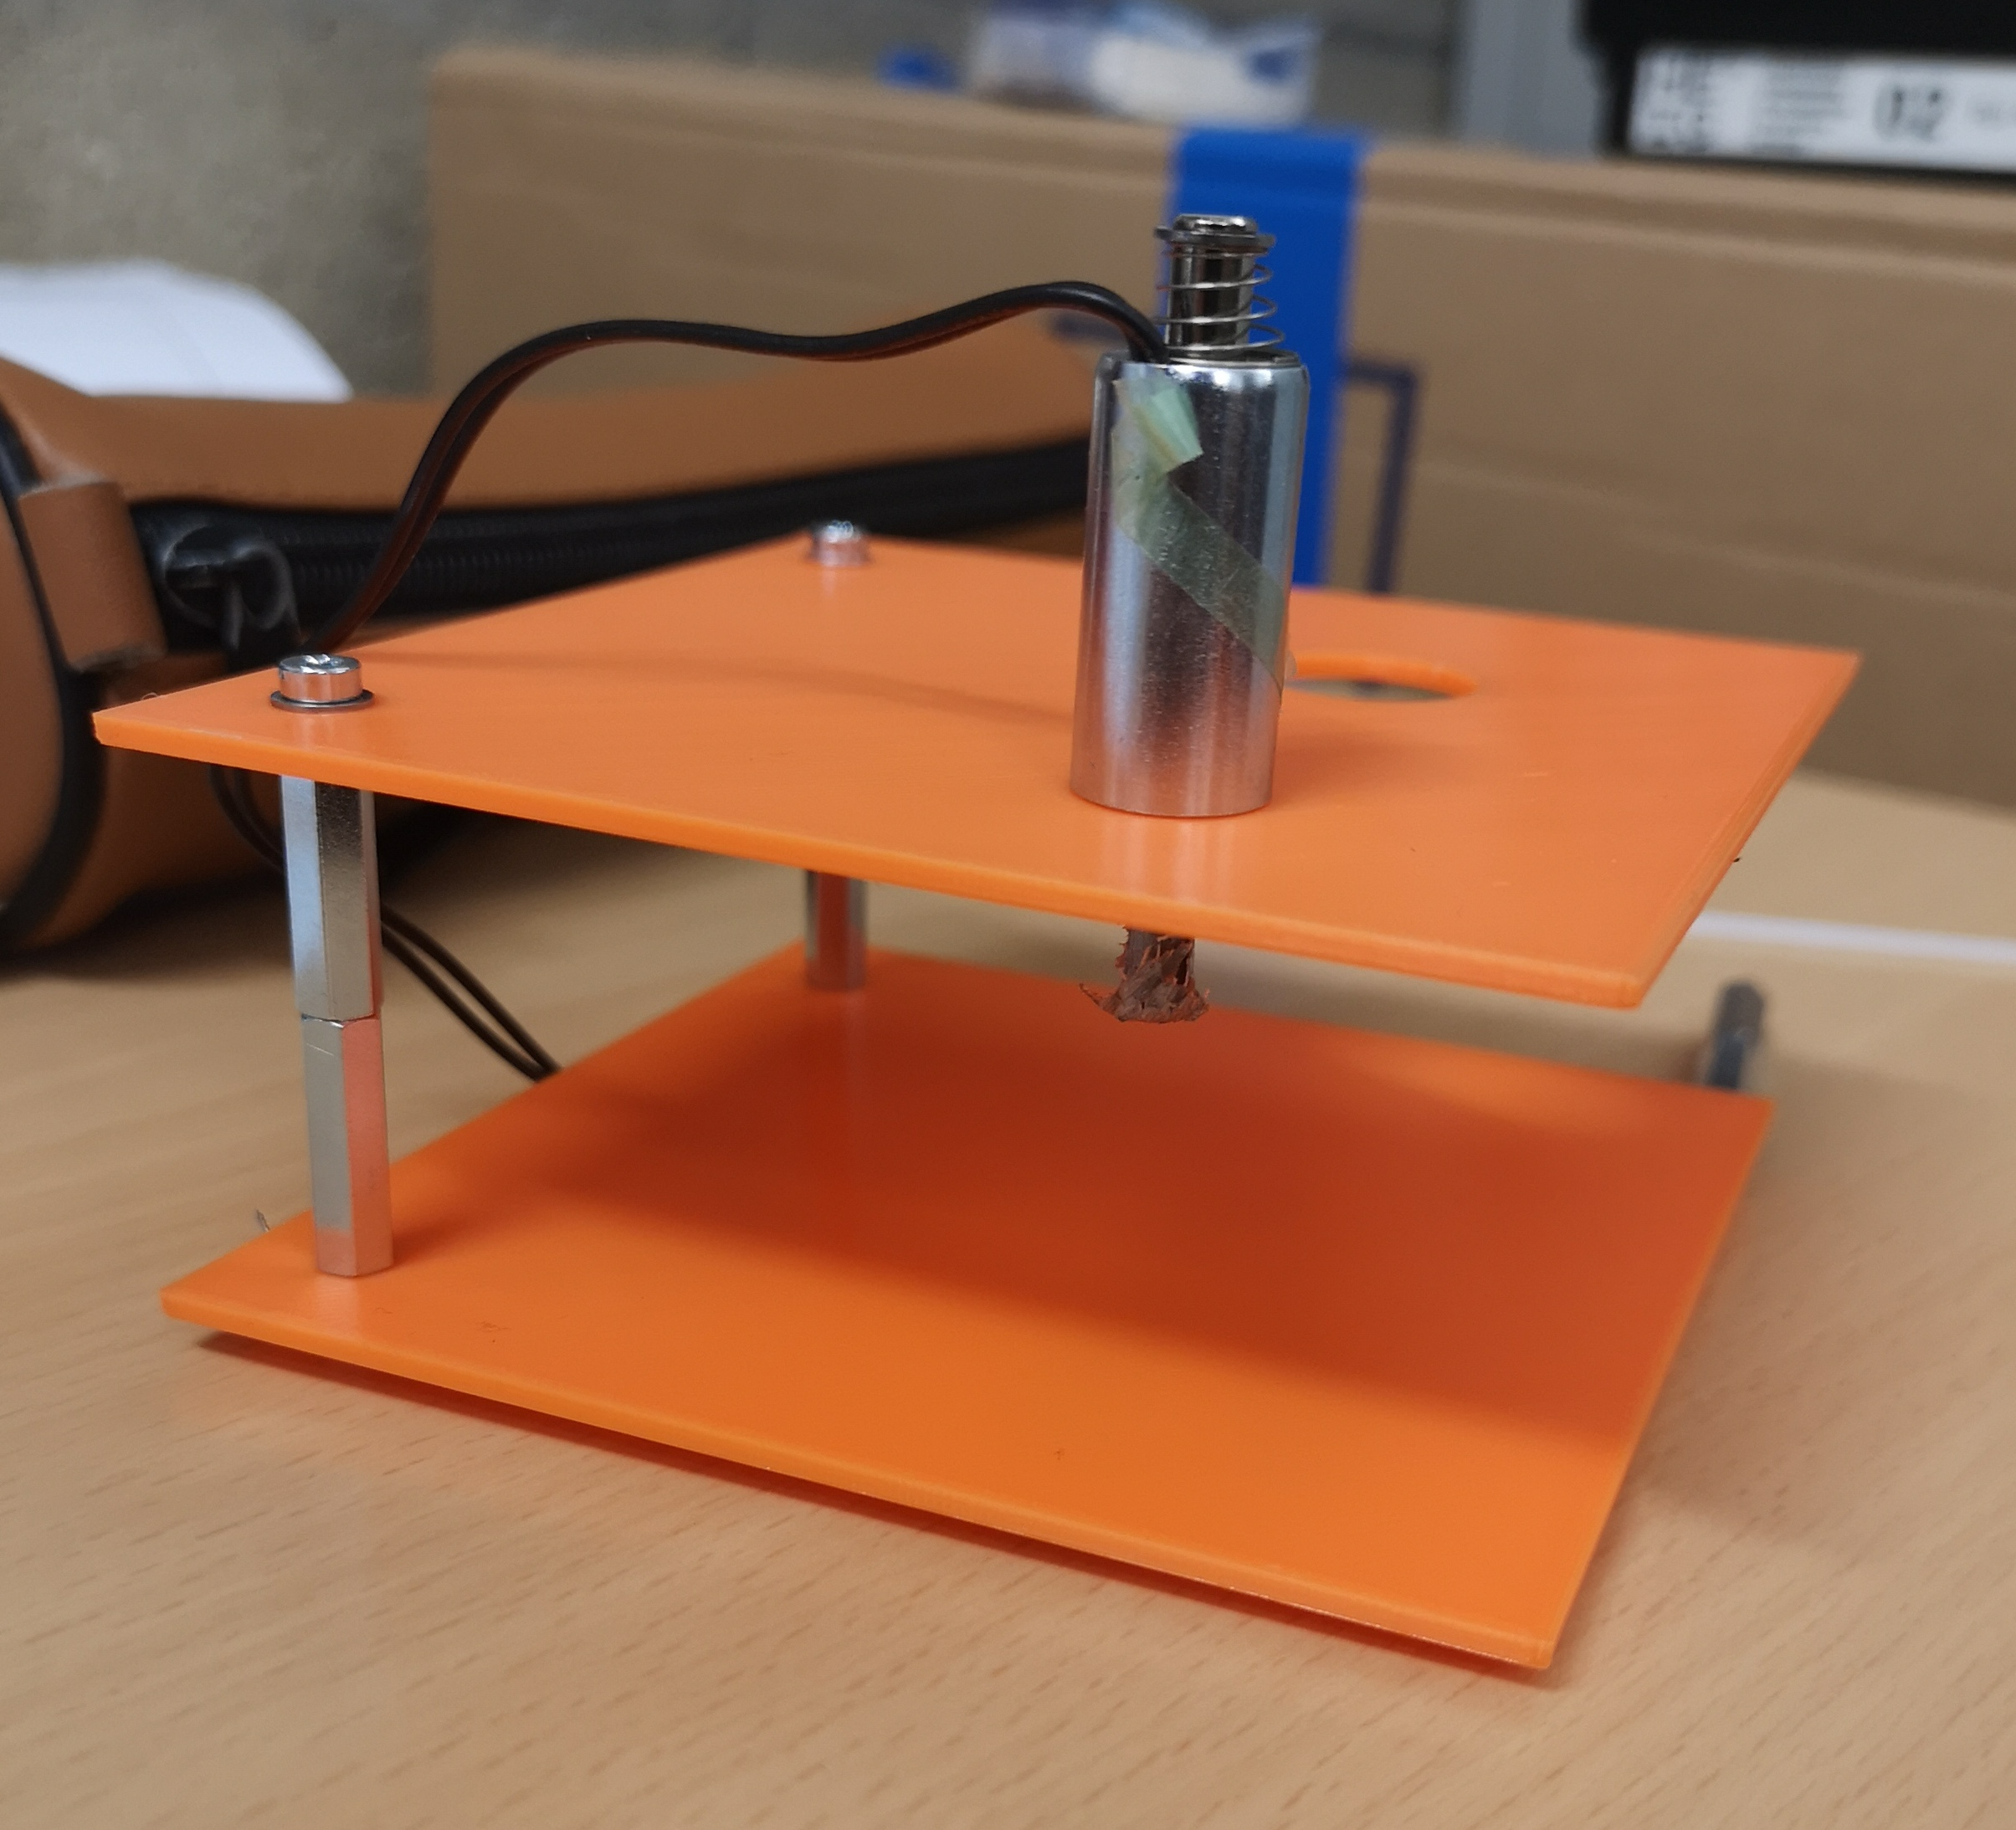
\includegraphics[width=10cm]{assets/figures/support_test_prehenseur.jpg}
    \caption{Système de préhension - Support de test}
\end{figure}

\begin{table}[h]
    \begin{center}
        \caption{Résultats du test de préhension}
        \begin{tabular}{|c|l|}
            Eléments       & Boutons \\ \hline
            Préhenseur 2N  & OUI-NON \\
            Préhenseur 11N & OUI-NON \\
        \end{tabular}
    \end{center}
\end{table}

\section{Supports}

\subsection{Support pour jeu de préhenseur magnétique}
\subsection{Support de la télécommande}

\section{Mesure de la vitesse}
Après que les traces d'hydrocarbures aient été détectées sur la route, il faut savoir quand ouvrir la section du semoir au bon moment. La distance entre la zone de détection et le semoir étant connue,
il est nécessaire de mesurer la vitesse afin de déterminer le temps après lequel il faut agir sur les ouvertures.
\subsection{Concept de mesure de vitesse}
Plusieurs solutions ont été envisagée:

\begin{itemize}
    \item Mesure par vision: L'idée serait d'utiliser l'image captée par la caméra et de la comparer avec l'image suivante. Sachant le temps entre deux images,
          la différence de position serait déterminer avec une corrélation. \underline{L'avantage} premier est que j'ai déjà la caméra, il n'y aurait pas besoin d'ajouter d'autres composants.
          \underline{Les inconvénients} sont les suivants, le filtre limitant les rayonnements visibles pourrait être problématique pour faire des corrélations, de plus, le temps de calcul nécessaire
          à une corrélation est trop grand, ce serait trop difficile de concilier efficacité de la cadence de traitement et mesure de la vitesse.
    \item Mesure par radar doppler: Vitesse radial, nécessite un obstacle, sur route peu adapté
    \item Mesure par capteur à effet Hall. L'idée est de fixer des aimants sur l'intérieur d'une des roues de la remorques de manière à connaître leurs placements.
          Ainsi, lorsque la roue est en mouvement, les aimants passent devant le capteur. Sachant les dimensions du pneus de la remorque, il serait possible de déterminer la vitesse en fonction de la fréquence d'activation du capteur.
          \underline{Avantages :} Peu coûteux, facile à mettre en place, nécessite seulement de configurer une routine d'interruption sur le \Gls{rpi4}. \underline{L'inconvénient} majeur est la difficulté à installer le tout.
    \item Mesure via une roue munie d'un tachymètre: L'idée consiste en l'ajout d'une roue
          inconvénients:
\end{itemize}

\subsection{Installation sur le semoir}

\section{Programme}
\subsection{Pilotage des vérins}
\subsection{Communication}